
%==============================


%fig 9.3 pg 361

\begin{figure}
\centering
\begin{tikzpicture}[x={(-0.5cm,-0.5cm)},y={(1cm,0cm)},z={(0cm,1cm)},declare function={f(\x)=2*sin(\x);}]
\draw[-stealth] (0,0,0) -- (2,0,0) node[left]{$x$};
\draw[-stealth] (0,0,0) -- (0,8,0) node[above]{$y$};
\draw[-stealth] (0,0,0) -- (0,0,2) node[left]{$z$};
%first 180 degrees
\pgfmathsetmacro{\t}{0}
\draw[thick] plot[domain=\t+0:\t+180,smooth]({f(\x)},{0.5 + \x/180},{0}); 
\foreach \x in {30,60,...,150}{\draw[-latex] ({0},{0.5+\x/180},{0}) --++ ({f(\x)},{0},{0});}
\draw[thick] plot[domain=\t+0:\t+180,smooth]({0},{0.5 + \x/180},{f(\x)});
\foreach \x in {30,60,...,150}{\draw[-latex] ({0},{0.5+\x/180},{0}) --++ ({0},{0},{f(\x)});}
%\draw[thick] plot[domain=180+0:180+180,smooth]({f(\x)},{0.5 + \x/180},{0}); 
% second 180 degrees
\pgfmathsetmacro{\t}{180}
\draw[thick] plot[domain=\t+0:\t+180,smooth]({f(\x)},{0.5 + \x/180},{0}); 
\foreach \x in {210,240,...,330}{\draw[-latex] ({0},{0.5+\x/180},{0}) --++ ({f(\x)},{0},{0});}
\pgfmathsetmacro{\t}{540}
\draw[thick] plot[domain=\t+0:\t+180,smooth]({f(\x)},{0.5 + \x/180},{0}); 
\foreach \x in {570,600,...,690}{\draw[-latex] ({0},{0.5+\x/180},{0}) --++ ({f(\x)},{0},{0});}
\pgfmathsetmacro{\t}{900}
\draw[thick] plot[domain=\t+0:\t+110,smooth]({f(\x)},{0.5 + \x/180},{0}); 
\foreach \x in {930,960,...,990}{\draw[-latex] ({0},{0.5+\x/180},{0}) --++ ({f(\x)},{0},{0});}
%now cutting the magnetic lines
\pgfmathsetmacro{\ct}{360}
\fill[fill=white] plot[domain=\ct+0:\ct+180,smooth]({0},{0.5 + \x/180},{f(\x)}) --cycle;
\draw[thick] plot[domain=\ct+0:\ct+180,smooth]({0},{0.5 + \x/180},{f(\x)});
\foreach \x in {390,410,...,530}{\draw[-latex] ({0},{0.5+\x/180},{0}) --++ ({0},{0},{f(\x)});}
\pgfmathsetmacro{\ct}{720}
\fill[fill=white] plot[domain=\ct+0:\ct+180,smooth]({0},{0.5 + \x/180},{f(\x)}) --cycle;
\draw[thick] plot[domain=\ct+0:\ct+180,smooth]({0},{0.5 + \x/180},{f(\x)});
\foreach \x in {730,760,...,870}{\draw[-latex] ({0},{0.5+\x/180},{0}) --++ ({0},{0},{f(\x)});}
%drawing to be cut portion of electric field
\pgfmathsetmacro{\t}{180}
\draw[thick] plot[domain=\t+0:\t+180,smooth]({0},{0.5 + \x/180},{f(\x)});
\foreach \x in {210,240,...,330}{\draw[-latex] ({0},{0.5+\x/180},{0}) --++ ({0},{0},{f(\x)});}
\pgfmathsetmacro{\t}{540}
\draw[thick] plot[domain=\t+0:\t+180,smooth]({0},{0.5 + \x/180},{f(\x)});
\foreach \x in {570,600,...,690}{\draw[-latex] ({0},{0.5+\x/180},{0}) --++ ({0},{0},{f(\x)});}
\pgfmathsetmacro{\t}{900}
\draw[thick] plot[domain=\t+0:\t+110,smooth]({0},{0.5 + \x/180},{f(\x)});
\foreach \x in {930,960,...,1010}{\draw[-latex] ({0},{0.5+\x/180},{0}) --++ ({0},{0},{f(\x)});}
%cutting electric field
\pgfmathsetmacro{\t}{360}
\fill[fill=white] plot[domain=\t+0:\t+180,smooth]({f(\x)},{0.5 + \x/180},{0}) --cycle;
\draw[thick] plot[domain=\t+0:\t+180,smooth]({f(\x)},{0.5 + \x/180},{0}); 
\foreach \x in {390,410,...,510}{\draw[-latex] ({0},{0.5+\x/180},{0}) --++ ({f(\x)},{0},{0});}
\pgfmathsetmacro{\t}{720}
\fill[fill=white] plot[domain=\t+0:\t+180,smooth]({f(\x)},{0.5 + \x/180},{0}) --cycle;
\draw[thick] plot[domain=\t+0:\t+180,smooth]({f(\x)},{0.5 + \x/180},{0}); 
\foreach \x in {750,780,...,870}{\draw[-latex] ({0},{0.5+\x/180},{0}) --++ ({f(\x)},{0},{0});}
\draw[-latex] (0.5,7,0) --++ (0,0.75,0) node[below,pos=0.5]{\RL{حرکت کا رخ}};
\draw[] ({f(90)}, {0.5+90/180}, {0}) node[pin=-130:{\RL{مقناطیسی میدان}}]{};
\draw[] ({0},{0.5+90/180},{f(90)}) node[pin=45:{\RL{برقی  میدان}}]{};
\end{tikzpicture}
\caption{
برقناطیسی موج۔
}
\label{
شکل_تابع_وقت_احتمال_برقناطیسی_ماج
}
\end{figure}




%==============================


%fig 9.4 pg 362

\begin{figure}
\centering
\begin{subfigure}{0.3\textwidth}
\centering
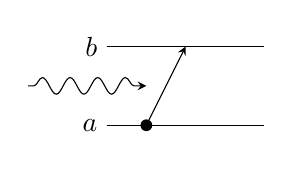
\begin{tikzpicture}
\draw[] (0,0.5) node[left]{$b$} --++ (2,0);
\draw[] (0,-0.5) node[left]{$a$} --++ (2,0);
\draw[-stealth] (0.5,-0.5) node[fill=black,circle,inner sep=1.5pt]{} -- (1,0.5);
\draw[-stealth,decorate,decoration={snake,amplitude=3pt,pre length=2pt,post length=3pt}] (-1,0) --++ (1.5,0);
\end{tikzpicture}
\caption{
جذب
}
\end{subfigure}\hfill
\begin{subfigure}{0.3\textwidth}
\centering
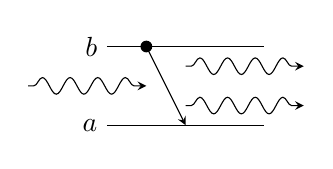
\begin{tikzpicture}
\draw[] (0,0.5) node[left]{$b$} --++ (2,0);
\draw[] (0,-0.5) node[left]{$a$} --++ (2,0);
\draw[-stealth] (0.5,0.5) node[fill=black,circle,inner sep=1.5pt]{} -- (1,-0.5);
\draw[-stealth,decorate,decoration={snake,amplitude=3pt,pre length=2pt,post length=3pt}] (-1,0) --++ (1.5,0);
\draw[-stealth,decorate,decoration={snake,amplitude=3pt,pre length=2pt,post length=3pt}] (1,0.25) --++ (1.5,0);
\draw[-stealth,decorate,decoration={snake,amplitude=3pt,pre length=2pt,post length=3pt}] (1,-0.25) --++ (1.5,0);
\end{tikzpicture}
\caption{
تحرک زدہ   اخراج
}
\end{subfigure}\hfill
\begin{subfigure}{0.3\textwidth}
\centering
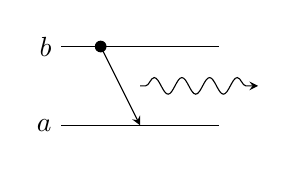
\begin{tikzpicture}
\draw[] (0,0.5) node[left]{$b$} --++ (2,0);
\draw[] (0,-0.5) node[left]{$a$} --++ (2,0);
\draw[-stealth] (0.5,0.5) node[fill=black,circle,inner sep=1.5pt]{} -- (1,-0.5);
\draw[-stealth,decorate,decoration={snake,amplitude=3pt,pre length=2pt,post length=3pt}] (1,0) --++ (1.5,0);
\end{tikzpicture}
\caption{
خود بخود  اخراج
}
\end{subfigure}
\caption{
روشنی  کا جوہر کے ساتھ تین قسم کے باہم عمل پائے جاتے ہیں۔ 
}
\label{
شکل_تابع_وقت_احتمال_روشنی_باہم_عمل
}
\end{figure}



%==============================


%fig 9.5 pg 364

\begin{figure}
\centering
\begin{tikzpicture}
\draw[-stealth,name path=px] (0,0) -- ++(-135:2.5) coordinate(kx) node[left]{$x$};
\draw[-stealth,name path=py] (0,0) --++ (0:4) coordinate(ky) node[below]{$y$};
\draw[-stealth,name path=pz] (0,0) -- ++(90:2) coordinate(kz) node[left]{$z$};
\draw[thick,-latex] (0,0)--++(-70:1.5) coordinate(kn) node[pos=0.5,right]{$\hat{n}$};
\draw[thick,-latex] (0,0)--++(20:3) coordinate(kp) node[pos=0.5,below right]{$\kvec{p}$};
\draw[] ([shift={(-135:0.5)}]0,0) arc (-135:-70:0.5) node[pos=0.5,below]{$\phi$};
\draw[] ([shift={(20:0.5)}]0,0) arc (20:90:0.5) node[pos=0.5,above]{$\theta$};
\path[name path=pn](kn)--++(-2,0);
\draw[dashed,name intersections={of={pn and px}}] (kn)--(intersection-1);
\path[name path=pp](kp)--++(-3,0);
\draw[dashed,name intersections={of={pp and pz}}] (kp)--(intersection-1);
\path[name path=ppp](kp)--++(0,-2);
\draw[dashed,name intersections={of={ppp and py}}] (kp)--(intersection-1);
\end{tikzpicture}
\caption{
محدد برائے \عددی{\abs{\kvec{p}\cdot\hat{n}}^2} کی اوسط زنی۔
}
\label{
شکل_تابع_وقت_اوسط_زنی_محدد
}
\end{figure}



%==============================


%fig 9.6 pg 374

\begin{figure}
\centering
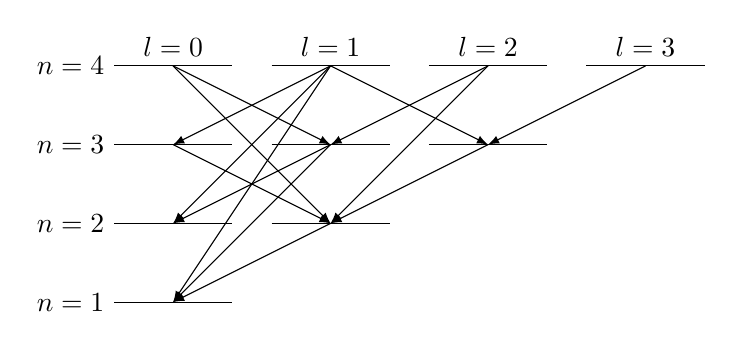
\begin{tikzpicture}
\pgfmathsetmacro{\kx}{1.5}
\pgfmathsetmacro{\ky}{1}
\pgfmathsetmacro{\ks}{0.5}
\draw[] (0,0) node[left]{$n=1$} --++ (\kx,0);
%
\draw[] (0,\ky) node[left]{$n=2$} --++ (\kx,0);
\draw[] (\kx+\ks,\ky) --++ (\kx,0);
%
\draw[] (0,2*\ky) node[left]{$n=3$} --++ (\kx,0);
\draw[] (\kx+\ks,2*\ky) --++ (\kx,0);
\draw[] (2*\kx+2*\ks,2*\ky) --++ (\kx,0);
%
\draw[] (0,3*\ky) node[left]{$n=4$} --++ (\kx,0) node[pos=0.5,above]{$l=0$};
\draw[] (\kx+\ks,3*\ky) --++ (\kx,0)node[pos=0.5,above]{$l=1$};
\draw[] (2*\kx+2*\ks,3*\ky) --++ (\kx,0)node[pos=0.5,above]{$l=2$};
\draw[] (3*\kx+3*\ks,3*\ky) --++ (\kx,0)node[pos=0.5,above]{$l=3$};
%
\draw[-latex] (\kx/2,3*\ky) --++ (\kx+\ks,-\ky);
\draw[-latex] (\kx/2,3*\ky) --++ (\kx+\ks,-2*\ky);
%
\draw[-latex] (\kx+\ks+\kx/2,3*\ky) --++ (-\kx-\ks,-\ky);
\draw[-latex] (\kx+\ks+\kx/2,3*\ky) --++ (-\kx-\ks,-2*\ky);
\draw[-latex] (\kx+\ks+\kx/2,3*\ky) --++ (-\kx-\ks,-3*\ky);
\draw[-latex] (\kx+\ks+\kx/2,3*\ky) --++ (\kx+\ks,-\ky);
%
\draw[-latex] (2*\kx+2*\ks+\kx/2,3*\ky) --++ (-\kx-\ks,-\ky);
\draw[-latex] (2*\kx+2*\ks+\kx/2,3*\ky) --++ (-\kx-\ks,-2*\ky);
%
\draw[-latex] (3*\kx+3*\ks+\kx/2,3*\ky) --++ (-\kx-\ks,-\ky);
%
\draw[-latex] (0*\kx+0*\ks+\kx/2,2*\ky) --++ (\kx+\ks,-\ky);
%
\draw[-latex] (1*\kx+1*\ks+\kx/2,2*\ky) --++ (-\kx-\ks,-\ky);
\draw[-latex] (1*\kx+1*\ks+\kx/2,2*\ky) --++ (-\kx-\ks,-2*\ky);
%
\draw[-latex] (2*\kx+2*\ks+\kx/2,2*\ky) --++ (-\kx-\ks,-1*\ky);
%
\draw[-latex] (1*\kx+1*\ks+\kx/2,1*\ky) --++ (-\kx-\ks,-1*\ky);
\end{tikzpicture}
\caption{
ہائیڈروجن کی اولین چار سطحوں کی اجازتی  تنزل۔
}
\label{
شکل_تابع_وقت_اضطراب_اجازتی_تنزل
}
\end{figure}



%==============================


%fig 10.1 pg 381

\begin{figure}
\centering
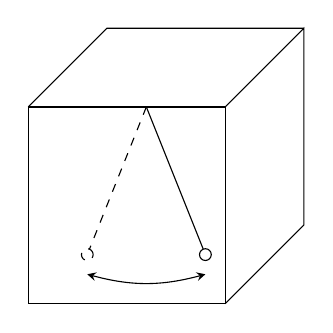
\begin{tikzpicture}[x={(-0.5cm,-0.5cm)},y={(1cm,0cm)},z={(0cm,1cm)}]
\pgfmathsetmacro{\kx}{2}
\pgfmathsetmacro{\ky}{2.5}
\pgfmathsetmacro{\kz}{2.5}
\draw[] (0,0,0) --++ (0,\ky,0) --++ (0,0,\kz) --++ (0,-\ky,0) --++ (0,0,-\kz);
\draw[] (0,\ky,0) --++ (-\kx,0,0) --++ (0,0,\kz) --++ (\kx,0,0);
\draw[] (0,0,\kz) --++ (-\kx,0,0) --++ (0,\ky,0);
\draw[] (0,0.6*\ky,\kz) --++ (0,0.3*\ky,-0.75*\kz) coordinate(a) node[circle,draw=black,fill=white, inner sep=1.5pt]{};
\draw[dashed] (0,0.6*\ky,\kz) --++ (0,-0.3*\ky,-0.75*\kz) coordinate(b) node[circle,draw=black,fill=white, inner sep=1.5pt]{};
\draw[stealth-stealth] (0,0.3*\ky,0.15*\kz) to [out=-15,in=-165] (0,0.9*\ky,0.15*\kz);
\end{tikzpicture}
\caption{
حرارت نا گزر حرکت: اگر ڈبے کو نہایت آہستہ ایک جگہ سے دوسری جگہ منتقل کیا جائے تب لٹکن اسی حیطہ کے ساتھ ابتدائی سطح کے متوازی سطح میں جھولتا ہے۔
}
\label{
شکل_حرارت_نا_گزر_آہستہ_منتقلی
}
\end{figure}



%===================================

%fig 10.2 pg 382

\begin{figure}
\centering
\begin{subfigure}{0.3\textwidth}
\centering
\begin{tikzpicture}
\fill[path fading=west,color=lgray] (-0.25,0) rectangle (0,1.25);
\fill[path fading=east,color=lgray] (1.5,0) rectangle (1.75,1.25);
\draw[-stealth] (-0.5,0) -- (3.5,0)node[below]{$x$};
\draw[-stealth] (0,-0.25) -- (0,1.5)node[right]{$\psi'(x)$};
\draw[very thick] plot [domain=0:180] ({\x/120},{sin(\x)}) node[below]{$a$};
\draw[] (3,0) node[below]{$2a$} --++ (0,0.1);
\draw[] (1.5,0) --++ (0,1.25);
\end{tikzpicture}
\caption{}
\end{subfigure}\hfill
\begin{subfigure}{0.3\textwidth}
\centering
\begin{tikzpicture}
\fill[path fading=west,color=lgray] (-0.25,0) rectangle (0,1.25);
\fill[path fading=east,color=lgray] (3,0) rectangle (3.25,1.25);
\draw[-stealth] (-0.5,0) -- (3.5,0)node[below]{$x$};
\draw[-stealth] (0,-0.25) -- (0,1.5)node[right]{$\psi'(x)$};
\draw[very thick] plot [domain=0:180] ({\x/60},{sin(\x)}) node[below]{$2a$};
\draw[] (1.5,0) node[below]{$a$} --++ (0,0.1);
\draw[] (3,0) --++ (0,1.25);
\end{tikzpicture}
\caption{}
\end{subfigure}\hfill
\begin{subfigure}{0.3\textwidth}
\centering
\begin{tikzpicture}
\fill[path fading=west,color=lgray] (-0.25,0) rectangle (0,1.25);
\fill[path fading=east,color=lgray] (3,0) rectangle (3.25,1.25);
\draw[-stealth] (-0.5,0) -- (3.5,0)node[below]{$x$};
\draw[-stealth] (0,-0.25) -- (0,1.5)node[right]{$\psi'(x)$};
\draw[very thick] plot [domain=0:180] ({\x/120},{sin(\x)}) node[below]{$a$} -- (3,0);
\draw[] (3,0) node[below]{$2a$};
\draw[] (3,0) --++ (0,1.25);
\end{tikzpicture}
\caption{}
\end{subfigure}
\caption{
(ا)  لامتناہی چکور کنواں کے زمینی حال  سے  ایک ذرہ ابتدا کرتا ہے، (ب)  اگر دیوار نہایت آہستہ حرکت کرے تب ذرہ اسی حال میں رہتا ہے، (ج) اگر دیوار تیزی سے حرکت کرے تب ذرہ لمحاتی طور پر ابتدائی حال میں رہتا ہے۔
}
\label{
شکل_حرارت_نا_گزر_ابتدائی_حال_کنواں_دیوار
}
\end{figure}


%==============================


%fig 10.3 pg 386

\begin{figure}
\centering
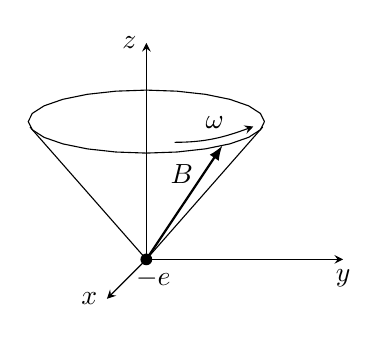
\begin{tikzpicture}
\pgfmathsetmacro{\a}{1.5}
\pgfmathsetmacro{\m}{0.7}
\pgfmathsetmacro{\b}{0.4}
\pgfmathsetmacro{\c}{1.75}
\draw[-stealth] (0,0) node[circle, fill=black,inner sep=1.5pt]{} node[below,xshift=0.25em]{$-e$} -- (-0.5,-0.5) node[left]{$x$};
\draw[-stealth] (0,0) -- (2.5,0) node[below]{$y$};
\draw[-stealth] (0,0) -- (0,2.75) node[left]{$z$};
\draw[] plot[domain=0:360] ({\a*cos(\x)},{\c+\b*sin(\x)});
%\draw[-stealth] plot[domain=290:350] ({\m*\a*cos(\x)},{\c+\m*\b*sin(\x)}) node[above left,yshift=-0.25em]{$\omega$};
\draw[thick, -latex] (0,0) -- ({\a*cos(310)},{\c+\b*sin(310)}) node[pos=0.75,left]{$\kvec{B}$};
\draw[] (0,0) -- ({\a*cos(190)},{\c+\b*sin(190)});
\draw[] (0,0) -- ({\a*cos(350)},{\c+\b*sin(350)});
\draw[-stealth] ({\m*\a*cos(290)},{\c+\m*\b*sin(290)})  to [out=0,in=-160] node[pos=0.5,above]{$\omega$} ++ (1,0.2);
\end{tikzpicture}
\caption{
مقناطیسی میدان  زاویائی  سمتی رفتار \عددی{\omega} سے مخروطی راہ جھاڑتا ہے (مساوات \حوالہء{10.24})۔   
}
\label{
شکل_حرارت_نا_گزر_مخروطی_راہ_جھاڑنا
}
\end{figure}



%==============================


%fig 10.4 pg 388

\begin{figure}
\centering
\pgfmathsetmacro{\a}{1.1}
\pgfmathsetmacro{\b}{sin(deg(\a))^2}
\begin{tikzpicture}[declare function={f(\x)=(sin(deg(\a))*sin(\x/2))^2;}]
\begin{axis}[axis lines=middle,xlabel={$t$},ylabel={$\abs{\langle\chi(t)|\chi_{-}(t)\rangle}^2$}, xtick={360,720,1080,1440}, xticklabels={$2\pi/\lambda$,$4\pi/\lambda$,$6\pi/\lambda$,$8\pi/\lambda$}, ytick={\b,1}, yticklabels={$(\tfrac{\omega\sin\alpha}{\lambda})^2$,$1$}, xlabel style={at={(current axis.right of origin)}, anchor={north}} ,ylabel style={at={(current axis.above origin)},anchor=west},enlargelimits]
\addplot [thick,domain=0:1500,samples=500] {f(x)};
\addplot [dashed] coordinates{(0,1)(1500,1)};
\addplot [dashed] coordinates{(0,\b)(1500,\b)};
\end{axis}
\end{tikzpicture}
\caption{
غیر حرارت نا گزر صورت   \عددی{(\omega\gg\omega_1)}   میں تحویلی  احتمال  (مساوات \حوالہء{10.34})۔
}
\label{
شکل_حرارت_نا_گزر_تحویلی_احتمال
}
\end{figure}



%==============================


%fig 10.5 pg 389

\begin{figure}
\centering
\pgfmathsetmacro{\r}{2}
\pgfmathsetmacro{\a}{40}
\pgfmathsetmacro{\b}{180-\a}
\begin{tikzpicture}
\draw[thick] (0,0) circle (\r);
\draw[thick] (-\r,0) to [out=-\a,in=-180] coordinate [pos=0.35] (tae) coordinate[pos=0.25](ta) (0,-0.75) to [out=0,in=-\b] coordinate [pos=0.65] (tbe) coordinate[pos=0.75] (tb) (\r,0);
\draw[thick] (ta) to [out=80,in=-150] node[pos=0.5,circle,fill=black,inner sep=1.5pt]{}coordinate[pos=0.5](kswabi) coordinate [pos=0.85](ka) coordinate [pos=0.1](kc) (0,\r);
\draw(kswabi)node[pin={-30:{\RL{صوابی}}}]{};
\draw[thick] (tb) to [out=100,in=-30] coordinate [pos=0.85](kb) coordinate [pos=0.1](kd) (0,\r);
\draw[-stealth] (-0.5,-0.75+0.2) to [out=-10,in=-170] (0.5,-0.75+0.2);
\draw[] (0,-0.75) node[below]{\RL{ارضی خط استوا}};
\draw[stealth-] ($(ta)+(-0.15,0.4)$) to [out=80,in=-110] ++ (0.15,0.5);
\draw[-stealth] ($(tb)+(0.15,0.4)$) to [out=100,in=-70] ++ (-0.15,0.5);
\draw[] (ka) to [out=-30,in=-150] node[pos=0.5,below]{$\theta$} (kb);
\RightAngle{(kc)}{(ta)}{(tae)}
\RightAngle{(kd)}{(tb)}{(tbe)}
\draw[] (0,\r+0.75) node[circle,fill=black,inner sep=1.5pt]{} --++ (0.2,-0.4) coordinate[pos=0.9](penb) node[pos=0.5,right]{\RL{رقاص}};
\draw[] (0,\r+0.75)  --++ (-0.3,-0.5) coordinate[pos=0.9](pena);
\draw[stealth-stealth] (pena) to [out=10,in=-150] (penb);
\end{tikzpicture}
\caption{
سطح زمین پر رقاص کی حرارت ناگزر منتقلی۔
}
\label{
شکل_حرارت_نا_گزر_سطح_زمین_منتقل
}
\end{figure}



%==============================


%fig 10.6 pg 389

\begin{figure}
\centering
\pgfmathsetmacro{\r}{2}
\begin{tikzpicture}
%\draw[thick] (-\r,-\r) grid (\r,\r);
%\draw[gray, step=0.1, thin] (-\r,-\r) grid (\r,\r);
\draw[thick] (0,0) circle (\r);
\draw[smooth, shading angle=130, ->-=0.15, ->-=0.5, ->-=0.65, ->-=0.85] plot [smooth] coordinates {(-1,1.25) (-1.25,1.25) (-1.75,0.5) (-1.25,0.75) (-0.25,0.5) (0.25,0.75) (-0.25,1)}--cycle;
\draw[] (-0.25,0.5) -- (0,0);
\draw[] (0.25,0.75) -- (0,0)coordinate[pos=0.5](kbb);
\draw[] (-1.75,0.5) -- (0,0)coordinate[pos=0.5](kaa);
\draw[stealth-] (kaa) to [out=-100,in=130] (0,-0.5);
\draw[stealth-] (kbb) to [out=-30,in=30] (0,-0.5)node[fill=white]{$\Omega$};
\end{tikzpicture}
\caption{
کرہ پر اختیاری راہ، ٹھوس زاویہ \عددی{\Omega} بناتا ہے۔
}
\label{
شکل_حرارت_نا_گزر_کرہ_پر_ٹھوس_زاویہ
}
\end{figure}



%==============================


%fig 10.7 pg 390

\begin{figure}
\centering
\pgfmathsetmacro{\r}{2}
\pgfmathsetmacro{\a}{0.8*\r}
\pgfmathsetmacro{\t}{90-acos(\a/\r)}
\pgfmathsetmacro{\b}{sqrt(\r^2-\a^2)}
\begin{tikzpicture}
\draw[] (0,0) circle (\r);
\draw[thick] (0,\a-0.05) circle (\b cm and 0.2cm);
\draw[] (0,0) node[fill=black,circle, inner sep=1.5pt]{} --++ (52.4:\r-0.1);
\draw[-stealth] (0,-0.25) -- (0,2.5) node[left]{$z$};
\draw[] ([shift={(90:0.5)}]0,0) arc (90:52.4:0.5) node[pos=0.5,above,xshift=0.25em]{$\theta_0$};
\end{tikzpicture}
\caption{
ایک دن کے دوران، فوقو رقاص کی راہ۔
}
\label{
شکل_حرارت_نا_گزر_فوقو_رقاص_ایک_دن
}
\end{figure}



%==============================


%fig 10.8 pg 393

\begin{figure}
\centering
\begin{tikzpicture}[scale=2]
%\draw[thick] (0,0) grid (3,2.5);
%\draw[thin,step=0.1] (0,0) grid (3,2.5);
\draw[thick,fill=lgray] plot[smooth cycle] coordinates{(0,1)(1,0.5)(2,1) (1.5,2)(0.5,1.75)};
\draw[] (0,1) node[left]{$C$};
\draw[fill=white] (0.5,1.25) --++ (0.3,0) --++ (0.1,0.2) --++ (-0.3,0) -- cycle; 
\draw[-latex, thick](0.7,1.35) --++ (0,1) node[left]{$\dif\kvec{a}$};
\draw[fill=white] (0.5,1) circle (3pt and 2pt);
\draw[fill=white] (1,0.7) circle (3pt and 2pt);
\draw[fill=white] (1.5,1) circle (3pt and 2pt);
\draw[fill=white] (1.25,1.5) circle (3pt and 2pt);
\draw[-stealth](0.5,1) to [out=90,in=-45] ++ (-0.5,1)node[left]{$\kvec{B}$};
\draw[-stealth](1,0.7) to [out=10,in=135] ++ (1,-0.5)node[right]{$\kvec{B}$};
\draw[-stealth](1.5,1) to [out=50,in=-160] ++ (1,0.5)node[right]{$\kvec{B}$};
\draw[-stealth](1.25,1.5) to [out=80,in=-170] ++ (1,0.5)node[right]{$\kvec{B}$};
\draw[] (0.6,0.8) to [out=-135,in=0] ++ (-0.5,-0.5) node[left]{$S$};
\end{tikzpicture}
\caption{
بند  منحنی  \عددی{C} کے بیچ سطح \عددی{S} سے گزرتا مقناطیسی بہاو۔
}
\label{
شکل_حرارت_نا_گزر_مقناطیسی_بہاو
}
\end{figure}



%==============================


%fig 10.9 pg 395
\begin{figure}
\centering
\begin{tikzpicture}
%\draw[thick] (0,0) grid (3,2.5);
%\draw[thin,step=0.1] (0,0) grid (3,2.5);
\draw[thick,fill=lgray,->-=0,->-=0.5] plot[smooth cycle] coordinates{(0,1)(1,0.5)(2,1) (1.5,2)(0.5,1.75)};
\draw[] (1.5,0.2) node[circle,fill=black,inner sep=1.5pt]{} circle (2);
\draw[-stealth, thick] (1.5,0.2) node[below]{$-e$} -- (1.9,0.85) node[pos=0.7,below right]{$\kvec{B}$};
\end{tikzpicture}
\caption{
مستقل  مقدار لیکن بدلتے رخ کا مقناطیسی میدان بند راہ پر چلتا ہے۔
}
\label{
شکل_حرارت_نا_گزر_مقناطیسی_میدان_بند_راہ
}
\end{figure}



%==============================


%fig 10.10 pg 398
\begin{figure}
\centering
\pgfmathsetmacro{\a}{0.75}
\pgfmathsetmacro{\b}{5}
\pgfmathsetmacro{\d}{0.05}
\begin{tikzpicture}[]
\draw[] (0,0) -- (0,\b);
\draw[] (\a,0) -- (\a,\b);
\draw[] (0,0) to [out=-90,in=-90] ++ (\a,0);
\draw[] (\a/2,\b) circle (\a/2 and \a/6);
\foreach \kk in {0.2,0.6,...,\b}{
\draw[] (-\d,\kk) to [out=-160,in=-10] ++ (\a+2*\d,0.1);}
\path (-\d,3.8) to [out=-160,in=-10] coordinate[pos=0.5](tpa)coordinate[pos=0.55](tpb) ++ (\a+2*\d,0.1);
\draw[] (-\d,3.8) node[left]{$I$};
\draw[-stealth,thick] (\a/2,\b) --++ (0,0.75) node[right]{$\kvec{B}$};
\draw[-stealth, very thick] (tpa) -- (tpb);
\draw[] (\a/2,-0.3) --++ (0,-0.3) coordinate[pos=0.5](bota);
\draw[] (\a,-0.3) --++ (0,-0.3) coordinate[pos=0.5](botb);
\draw[-stealth] (bota) -- (botb) node[pos=0.5,below]{$a$};
\draw[very thick] plot[domain=105:435]({\a/2+2*cos(\x)},{\b/2+0.55*sin(\x)});
\draw  ({\a/2+2*cos(220)},{\b/2+0.55*sin(220)})node[circle,fill=black,inner sep=1.5pt]{}coordinate(kkk) node[below]{$q$};
\draw[-latex,shorten >=2pt](\a/2,\b/2)--(kkk) node[pos=0.75, above]{$b$};
\end{tikzpicture}
\caption{
ایک دائرہ ، جس کے اندر سے ایک لمبا پیچواں برقی مقناطیس گزرتا ہو، پر ایک باردار ذرہ حرکت کرتا ہے۔ 
}
\label{
شکل_حرارت_نا_گزر_پیچواں_دائرہ_حرکت
}
\end{figure}




%==============================


%fig 10.11 pg 400
\begin{figure}
\centering
\pgfmathsetmacro{\a}{0.75}
\pgfmathsetmacro{\b}{5}
\pgfmathsetmacro{\d}{0.05}
\begin{tikzpicture}[]
\draw[very thick, ->-=0.1,->-=0.35,->-=0.75] (-3,\b/2+0.1) to [out=0,in=180]  (\a/2,\b/2+0.75) to [out=0,in=180] (3+\a,\b/2);
\draw[very thick, ->-=0.1,->-=0.35,->-=0.75,-stealth] (-3,\b/2-0.1) to [out=0,in=180]  (\a/2,\b/2-0.75) to [out=0,in=180] (3+\a,\b/2);
\fill[white] (-0.15,\b/2) rectangle (\a+0.15,\b/2+1);
\draw[] (-2,\b/2-0.25) node[pin={-130:{\RL{تقسین شدہ شعاع}}}]{};
\draw[] (\a+2,\b/2-0.25) node[pin={-30:{\RL{دوبارہ ملاپ شعاع}}}]{};
\draw[] (0,0) -- (0,\b);
\draw[] (\a,0) -- (\a,\b);
\draw[] (0,0) to [out=-90,in=-90] ++ (\a,0);
\draw[] (\a/2,\b) circle (\a/2 and \a/6);
\foreach \kk in {0.2,0.6,...,\b}{
\draw[] (-\d,\kk) to [out=-160,in=-10] ++ (\a+2*\d,0.1);}
\path (-\d,3.8) to [out=-160,in=-10] coordinate[pos=0.5](tpa)coordinate[pos=0.55](tpb) ++ (\a+2*\d,0.1);
\draw[] (-\d,3.8) node[left]{$I$};
\draw[-stealth,thick] (\a/2,\b) --++ (0,0.75) node[right]{$\kvec{B}$};
\draw[-stealth, very thick] (tpa) -- (tpb);
\draw[](\a/2,0)node[below,yshift=-1em]{\RL{پیچواں برقی مقناطیس}};
\draw[-stealth] plot[domain=120:415]({\a/2+1*cos(\x)},{\b/2+0.25*sin(\x)});
\draw[] (\a/2+1,\b/2) node[right]{$\kvec{A}$};
\end{tikzpicture}
\caption{
اہارانو و بوہم اثر: ایلکٹران شعاع تقسیم ہو کر  آدھا حصہ لمبے پیچواں برقی مقناطیس کے ایک طرف اور دوسرا حصہ دوسرے طرف سے گزرتا ہے۔ 
}
\label{
شکل_حرارت_نا_گزر_اہارانووبوہم
}
\end{figure}

%==============================


%fig 10.12 pg 401
\begin{figure}
\centering
\pgfmathsetmacro{\a}{0.75}
\pgfmathsetmacro{\b}{5}
\pgfmathsetmacro{\la}{1.5}
\pgfmathsetmacro{\lb}{1.5}
\pgfmathsetmacro{\lc}{1}
\begin{tikzpicture}[]
\draw[] (0,0) -- (0,\b);
\draw[] (\a,0) -- (\a,\b);
\draw[] (0,0) to [out=-90,in=-90] ++ (\a,0);
\draw[] (\a/2,\b) circle (\a/2 and \a/6);
\draw[] (3,3) coordinate(fa) --++ (\la,0) --++ (0, \lb) --++ (-\la,0) --++(0,-\lb);
\draw[] (3,3) ++ (\la,0) --++ (45:\lc) --++ (0,\lb) coordinate(fb) --++ (-\la, 0) --++ (45:-\lc);
\draw[] (3,3) ++ (\la,\lb) --++ (45:\lc);
\draw[] (\a/2,2) --++ (-0.2,-0.2);
\draw[] (\a/2,2) --++ (0.25,0);
\draw[] (\a/2,2) --++ (0,0.25);
\draw[-stealth,shorten >=2pt] (\a/2,2) -- ($(fa)!0.5!(fb)$) node[pos=0.5,above]{$\kvec{R}$} coordinate(tipa); 
\draw[-latex] (\a/2,2) -- ($(3+\la,3+\lb/5)+(45:\lc/3)$) node[pos=0.5,below]{$\kvec{r}$} coordinate(tipb); 
\draw[-stealth] (tipa)node[circle,fill=black,inner sep=1.5pt]{} -- (tipb) node[pos=0.25,pin={[pin distance=1.25cm,pin edge=-]30:{$(\kvec{r}-\kvec{R})$}}]{};
\end{tikzpicture}
\caption{
مخفیہ \عددی{V(\kvec{r}-\kvec{R})} ایک ذرہ کوڈبیہ میں  مقید کیے ہوئے ہے۔
}
\label{
شکل_حرارت_نا_گزر_مقید_ذرہ_ڈبیہ
}
\end{figure}
